\section{Proof of Some Basic Properties}
\label{sec:app-a}



\subsection{Proof of Lemma \ref{lemma3.6}}\label{pro-lemma}  

\paragraph{\emph{Non}-expansive.} Function is convexity and $\beta$-smoothness that implies 
\begin{equation}\label{eq:app2.2}
     \begin{aligned}
      \langle \nabla F(\theta_1) -\nabla F(\theta_2), \theta_1 - \theta_2 \rangle \geq \frac{1}{\beta} \Vert \nabla F(\theta_1) -\nabla F(\theta_2)\Vert^2 .
     \end{aligned}
\end{equation}
If $\eta \leq \frac{2}{\beta}$, we conclude that
\begin{equation}\label{eq:app2.3}
     \begin{aligned}
      \Vert \theta_{T+1} - &\theta_{T+1}^{\prime}\Vert = \sqrt{\Vert \theta_{T} - \alpha \nabla F(\theta_{T}) - \theta_{T}^{\prime} + \eta \nabla F(\theta_{T}^{\prime})\Vert^2}  \\
      &=\sqrt{\Vert \theta_{T} - \theta_{T}^{\prime} \Vert^2 - 2\eta\langle \nabla F(\theta_{T}) -\nabla F(\theta_{T}^{\prime}), \theta_T- \theta_T^{\prime} \rangle +\eta^2 \Vert \nabla F(\theta_{T}) - \nabla F(\theta_{T}^{\prime})\Vert^2} \\
      &\leq \sqrt{\Vert \theta_T- \theta_T^{\prime}\Vert^2 - \left(\frac{2\eta}{\beta} -\eta^2 \right) \Vert \nabla F(\theta_{T}) -\nabla F(\theta_{T}^{\prime})\Vert^2} \\
      &\leq \Vert \theta_T- \theta_T^{\prime}\Vert.
     \end{aligned}
\end{equation}


\section{Generalization Bound under Convexity}\label{sec:app-convex}

\subsection{Proof of Theorem \ref{thm:sgd-WD}}\label{sec:app-thm4.1}
Next, we first present the generalization bound for SGD-WD based on the formulation \eqref{SGD-DW-rules}:
\begin{equation}
  \begin{aligned}
   \theta_t =  \theta_{t-1} - \eta (\nabla F(\theta_{t-1},z_{t}) + \lambda \theta_{t-1} ) = (1-\lambda \eta) \theta_{t-1} - \eta \nabla F(\theta_{t-1},z_{t}).
  \end{aligned}
 \end{equation}

First, we consider that the different samples are selected to update with probability $\frac{1}{n}$ at the step $T+1$.  
\begin{equation}
  \begin{aligned}
   \Vert \theta_t -\theta_t^{\prime} \Vert &= \Vert (1-\lambda \eta) (\theta_{t-1} - \theta_{t-1}^{\prime}) + \eta (\nabla F(\theta_{t-1}^{\prime},z_{t}^{\prime}) - \nabla F(\theta_{t-1},z_{t}))\Vert\\
    &\leq (1-\lambda \eta)\Vert\theta_{t-1} - \theta_{t-1}^{\prime}\Vert + 2 \eta G,
  \end{aligned}
 \end{equation}
where the inequality follows from the triangle inequality, Lipschitz assumption for the target function $F$.

Second, the same samples are selected with probability $1-\frac{1}{n}$ at step $T+1$. 
 \begin{equation}
  \begin{aligned}
   \Vert \theta_t -\theta_t^{\prime} \Vert &= \Vert (1-\lambda \eta) (\theta_{t-1} - \theta_{t-1}^{\prime}) + \eta (\nabla F(\theta_{t-1}^{\prime},z_{t}^{\prime}) - \nabla F(\theta_{t-1},z_{t}))\Vert\\
    &\leq (1-\lambda \eta)\Vert\theta_{t-1} - \theta_{t-1}^{\prime}\Vert.
  \end{aligned}
 \end{equation}
This is because the objective function is convex and smooth, enabling the entire update process to exhibit $(1-\lambda\eta)$-expansion. As shown in the following analysis: Function is convexity and $\beta$-smoothness, if $\eta \leq \frac{2}{2\lambda+\beta}$, we conclude that

\begin{equation}\label{eq:app2.3}
     \begin{aligned}
      &\Vert \theta_{T+1} - \theta_{T+1}^{\prime}\Vert = \sqrt{\Vert (1-\lambda\eta)\theta_{T} - \eta \nabla F(\theta_{T}) - (1-\lambda\eta)\theta_{T}^{\prime} + \eta \nabla F(\theta_{T}^{\prime})\Vert^2}  \\
      &=\!\sqrt{\!(1-\lambda\eta)^2\Vert \theta_{T} \!-\! \theta_{T}^{\prime} \Vert^2 \!-\! 2\eta (1\!-\!\lambda\eta)\langle \nabla F(\theta_{T}) \!-\!\nabla F(\theta_{T}^{\prime}), \theta_T \!-\! \theta_T^{\prime} \rangle \!+\!\eta^2 \Vert \nabla F(\theta_{T}) \!-\! \nabla F(\theta_{T}^{\prime})\Vert^2} \\
      &\leq \sqrt{(1-\lambda\eta)^2\Vert \theta_T- \theta_T^{\prime}\Vert^2 - \left(\frac{2\eta (1-\lambda\eta)}{\beta} -\eta^2 \right) \Vert \nabla F(\theta_{T}) -\nabla F(\theta_{T}^{\prime})\Vert^2} \\
      &\leq (1-\lambda\eta)\Vert \theta_T- \theta_T^{\prime}\Vert,
     \end{aligned}
\end{equation}
where the first inequality imposes stricter requirements on the learning rate of $\frac{2\eta (1-\lambda\eta)}{\beta} -\eta^2 \geq 0$.

Let $\delta_{T}=\Vert\theta_T- \theta_T^{\prime}\Vert$, we obtain the expectation based on the above analysis 
  \begin{equation}
  \begin{aligned}
    \mathbb{E}\left[\delta_{T}\right] &\leq (1-\frac{1}{n})(1-\lambda \eta)\mathbb{E}\left[\delta_{T-1}\right] + \frac{1}{n}\left((1-\lambda \eta)\mathbb{E}\left[\delta_{T-1}\right] + 2\eta G\right)\\
    &\leq (1-\lambda \eta)\mathbb{E}\left[\delta_{T-1}\right] + \frac{2\eta G}{n}
  \end{aligned}
 \end{equation}
recursively, we can get 
    \begin{equation}
     \begin{aligned}
      \mathbb{E}\left[\delta_{T}\right] \leq \frac{2\eta G}{n} \sum_{t=0}^{T}(1-\lambda \eta)^t \leq \frac{2G}{\lambda n}.
     \end{aligned}
    \end{equation}

Plugging this back into Eq.~\eqref{convex-basic}, we obtain
 \begin{equation}\label{eq:2.2.1}
  \epsilon_{gen} = \epsilon_{stab} = \mathbb{E}\vert L(\theta_T;z) - L(\theta^{\prime}_T;z)\vert \leq \frac{2G^2}{\lambda n}.
 \end{equation}
And we finish the proof.

\subsection{Proof of Theorem \ref{thm:sgdm}}\label{sec:app-thm:sgdm}

We set $u_t = m_t$ and $\lambda=0$ in Eq. \ref{SGD-DW-rules}, yielding the following update formula for SGDM: 
\begin{equation}
  \begin{aligned}
   \theta_t = \theta_{t-1} - \eta m_t = \theta_{t-1} - \eta (\beta m_{t-1}+(1-\beta)\nabla F(\theta_{t-1},z_t)),
  \end{aligned}
 \end{equation}
where $m_t = \beta m_{t-1}+(1-\beta)\nabla F(\theta_{t-1},z_t)$ denotes the momentum.

As demonstrated in the proof above, at step T+1, we need to consider two distinct sampling scenarios. First, we consider that the different samples are selected with probability $\frac{1}{n}$ at step $T+1$.  
\begin{equation}\label{sgdm}
  \begin{aligned}
   \Vert \theta_t -\theta_t^{\prime} \Vert &= \Vert  (\theta_{t-1} - \theta_{t-1}^{\prime}) + \eta (m_t - m_t^{\prime})\Vert\\
   &= \Vert (\theta_{t-1} - \theta_{t-1}^{\prime}) + \eta (1-\beta)(\nabla F(\theta_{t-1}^{\prime},z_{t}^{\prime}) - \nabla F(\theta_{t-1},z_{t})) + \eta \beta(m_{t-1} - m_{t-1}^{\prime})\Vert\\
    &\leq \Vert\theta_{t-1} - \theta_{t-1}^{\prime}\Vert + 2\eta(1-\beta)G + 2\eta \beta\Vert m_{t-1}\Vert,
  \end{aligned}
 \end{equation}
where the first inequality follows from the triangle inequality and the Lipschitz assumption.

Under this setting, unlike SGD, we need to find the upper bound for $\mathbb{E} \Vert m_t\Vert$. Then, we have 
\begin{equation}\label{m-t}
  \begin{aligned}
   \mathbb{E} \Vert m_t\Vert &=  \mathbb{E} \Vert (1-\beta)m_{t-1} + \beta \nabla F(\theta_{t-1},z_t)\Vert \\
   &\leq (1-\beta)\mathbb{E} \Vert m_{t-1} \Vert + \beta \Vert\nabla F(\theta_{t-1},z_t)\Vert \\
   &= (1-\beta)\mathbb{E} \Vert (1-\beta)m_{t-2} + \beta \nabla F(\theta_{t-2},z_{t-1}) \Vert + \beta \Vert\nabla F(\theta_{t-1},z_t)\Vert \\
   &\cdots \\
   &\leq \sum_{i=0}^{t}(1-\beta)^i\beta G = G(1-(1-\beta)^t),
  \end{aligned}
 \end{equation}

Therefore, combining Eq. \ref{sgdm} and \ref{m-t}, we have
\begin{equation}
  \begin{aligned}
   \Vert \theta_t -\theta_t^{\prime} \Vert \leq \Vert\theta_{t-1} - \theta_{t-1}^{\prime}\Vert + 2\eta \tau_\beta G,
  \end{aligned}
 \end{equation}
where $\tau_\beta\in(0,1)$ is a very small constant dependent on $\beta$, with $\tau_\beta=[1-(1-\beta)^t]\beta+(1-\beta)$. In fact, as $t\rightarrow \infty$, $\tau_\beta \rightarrow 1$. We retain the explicit expression of this coefficient to reflect its dependence on the parameter $\beta$.

Second, the same samples are selected to update with probability $1-\frac{1}{n}$ at the step $T+1$. 
 \begin{equation}
  \begin{aligned}
   \Vert \theta_t -\theta_t^{\prime} \Vert &= \Vert (\theta_{t-1} - \theta_{t-1}^{\prime}) + \eta (1-\beta)(\nabla F(\theta_{t-1}^{\prime},z_{t}^{\prime}) - \nabla F(\theta_{t-1},z_{t})) + \eta \beta(m_{t-1} - m_{t-1}^{\prime})\Vert\\
    &\leq \Vert\theta_{t-1} - \theta_{t-1}^{\prime}\Vert,
  \end{aligned}
 \end{equation}
where the first inequality is due to the non-expansive property of a convex function, as shown in the following proof.

We first determine the learning rate that satisfies the non-expansion property for the objective function.
\begin{equation}\label{eq:app2.3}
     \begin{aligned}
      &\Vert \theta_{T+1} - \theta_{T+1}^{\prime}\Vert = \Vert ((\theta_{T}-\theta_{T}^{\prime}) + \eta(1-\beta) (\nabla F(\theta_{T})-\nabla F(\theta_{T}^{\prime}))
      +\eta\beta(m_t-m_t^{\prime})\Vert  \\
      &\leq \sqrt{\Vert \theta_{T} \!-\! \theta_{T}^{\prime} \Vert^2 \!-\! 2\eta (1\!-\!\beta)\langle \nabla F(\theta_{T})\! -\!\nabla F(\theta_{T}^{\prime}), \theta_T \!-\! \theta_T^{\prime} \rangle \!+\!\eta^2(1 \!-\!\beta)^2 \Vert \nabla F(\theta_{T}) \!-\! \nabla F(\theta_{T}^{\prime})\Vert^2}\\& + \eta\beta\Vert m_t-m_t^{\prime}\Vert\\
      &\leq \sqrt{\Vert \theta_T- \theta_T^{\prime}\Vert^2 - \left(\frac{2\eta (1-\beta)}{L} -\eta^2(1-\beta)^2 \right) \Vert \nabla F(\theta_{T}) -\nabla F(\theta_{T}^{\prime})\Vert^2} + 2\eta\beta G \\
      &\leq \Vert \theta_T- \theta_T^{\prime}\Vert - \frac{\left(\frac{2\eta (1-\beta)}{L} -\eta^2(1-\beta)^2 \right) \Vert \nabla F(\theta_{T}) -\nabla F(\theta_{T}^{\prime})\Vert^2}{2\Vert \theta_T- \theta_T^{\prime}\Vert} + 2\eta\beta G,
     \end{aligned}
\end{equation}
where the last inequality comes from the first-order Taylor expansion $\sqrt{a^2-b}\leq a-\frac{b}{2a}$. 

Let $\frac{\left(\frac{2\eta (1-\beta)}{L} -\eta^2(1-\beta)^2 \right) \Vert \nabla F(\theta_{T}) -\nabla F(\theta_{T}^{\prime})\Vert^2}{2\Vert \theta_T- \theta_T^{\prime}\Vert} \geq  2\eta\beta G$, we can further obtain the desired property $\Vert \theta_{T+1} - \theta_{T+1}^{\prime}\Vert \leq \Vert \theta_T- \theta_T^{\prime}\Vert$, which requires us to specify a learning rate that satisfies the condition. Rearranging this inequality, we get
\begin{equation}
\begin{aligned}
4\eta \beta G \Vert \theta_T - \theta_T^{\prime}\Vert &\leq (\frac{2\eta (1-\beta)}{L} - \eta^2(1-\beta)^2)\Vert \nabla F(\theta_T) - \nabla F(\theta_T^{\prime})\Vert^2 \\
& \leq (\frac{2\eta (1-\beta)}{L} - \eta^2(1-\beta)^2)L^2\Vert \theta_T - \theta_T^{\prime}\Vert^2.
\end{aligned}
\end{equation}
To ensure that the dominating term $\Vert \theta_T - \theta_T^{\prime}\Vert \leq \Vert \nabla F(\theta_T) - \nabla F(\theta_T^{\prime})\Vert^2$ in the first inequality is satisfied, we use property $\Vert \theta_T - \theta_T^{\prime}\Vert \leq \frac{1}{\mu}\Vert \nabla F(\theta_T) - \nabla F(\theta_T^{\prime})\Vert$ of the strong convexity assumption to guarantee this. The second inequality follows from the $L$-smooth assumption. Rearranging the above inequality, we have 
\begin{equation}
\begin{aligned}
\eta\leq\frac{2}{L(1-\beta)}-\frac{4\beta G}{L^2(1-\beta)^2\Vert \theta_T - \theta_T^{\prime}\Vert}\leq\frac{2}{L(1-\beta)},
\end{aligned}
\end{equation}
where the last inequality follows because $G,L,\Vert\cdot\Vert >0,0<\beta<1$. Moreover, in practice $\Vert \theta_T - \theta_T^{\prime}\Vert$ is often large enough, which ensure $\frac{2}{L(1-\beta)} - \frac{4\beta G}{L^2(1-\beta)^2\Vert \theta_T - \theta_T^{\prime}\Vert}>0$.

Finally, we obtain the desired learning rate $\eta \leq \frac{2}{L(1-\beta)}$. Then, we have the conclusion the target function is convexity and $L$-smoothness, if $\eta \leq \frac{2}{L(1-\beta)}$, we conclude that $\Vert \theta_{T+1} - \theta_{T+1}^{\prime}\Vert \leq \Vert \theta_T- \theta_T^{\prime}\Vert$. And, we obtain the expectation based on the above analysis 
  \begin{equation}
  \begin{aligned}
    \mathbb{E}\left[\delta_{T}\right] &\leq (1-\frac{1}{n})\mathbb{E}\left[\delta_{T-1}\right] + \frac{1}{n}\left(\mathbb{E}\left[\delta_{T-1}\right] + 2\eta\tau_{\beta} G\right)\\
    &\leq \mathbb{E}\left[\delta_{T-1}\right] + \frac{2\eta\tau_{\beta} G}{n}
  \end{aligned}
 \end{equation}
recursively, we can get 
    \begin{equation}
     \begin{aligned}
      \mathbb{E}\left[\delta_{T}\right] \leq \frac{2\eta\tau_{\beta} G T}{n} .
     \end{aligned}
    \end{equation}

Plugging this back into Eq.~\eqref{convex-basic}, we obtain
 \begin{equation}\label{eq:2.2.1}
  \epsilon_{gen} = \epsilon_{stab} = \mathbb{E}\vert F(\theta_T;z) - F(\theta^{\prime}_T;z)\vert \leq \frac{2\tau_{\beta}\eta G^2 T}{n}.
 \end{equation}
And we finish the proof.

\subsection{Proof of Theorem \ref{thm:sgdm-WD}}\label{sec:app-thm:sgdm-wd}

We set $u_t = m_t$ in Eq. \ref{SGD-DW-rules}, yielding the following update formula for SGDM-WD: 
\begin{equation}
  \begin{aligned}
   \theta_t = & \theta_{t-1} - \eta (m_t + \lambda \theta_{t-1} ) = (1-\lambda \eta) \theta_{t-1} - \eta m_t \\
   = & (1-\lambda \eta) \theta_{t-1} - \eta (\beta m_{t-1}+(1-\beta)\nabla F(\theta_{t-1},z_t)),
  \end{aligned}
 \end{equation}
where $m_t = \beta m_{t-1}+(1-\beta)\nabla F(\theta_{t-1},z_t)$ denotes the momentum.

As demonstrated in the proof above, at step T+1, we need to consider two distinct sampling scenarios. First, we consider that the different samples are selected with probability $\frac{1}{n}$ at step $T+1$.  
\begin{equation}
  \begin{aligned}
   \Vert &\theta_t -\theta_t^{\prime} \Vert = \Vert (1-\lambda \eta) (\theta_{t-1} - \theta_{t-1}^{\prime}) + \eta (m_t - m_t^{\prime})\Vert\\
   &= \Vert (1-\lambda \eta) (\theta_{t-1} - \theta_{t-1}^{\prime}) + \eta (1-\beta)(\nabla F(\theta_{t-1}^{\prime},z_{t}^{\prime}) - \nabla F(\theta_{t-1},z_{t})) + \eta \beta(m_{t-1} - m_{t-1}^{\prime})\Vert\\
    &\leq (1-\lambda \eta)\Vert\theta_{t-1} - \theta_{t-1}^{\prime}\Vert + 2\eta(1-\beta)G + 2\eta \beta\Vert m_{t-1}\Vert \\
    &\leq (1-\lambda \eta)\Vert\theta_{t-1} - \theta_{t-1}^{\prime}\Vert + 2\eta \tau_\beta G,
  \end{aligned}
 \end{equation}
where the first inequality follows from the triangle inequality and the Lipschitz assumption.

% Under this setting, unlike SGD-WD, we need to find the upper bound for $\mathbb{E} \Vert m_t\Vert$. Then, we have 
% \begin{equation}\label{m-t}
%   \begin{aligned}
%    \mathbb{E} \Vert m_t\Vert &=  \mathbb{E} \Vert (1-\beta)m_{t-1} + \beta \nabla F(\theta_{t-1},z_t)\Vert \\
%    &\leq (1-\beta)\mathbb{E} \Vert m_{t-1} \Vert + \beta \Vert\nabla F(\theta_{t-1},z_t)\Vert \\
%    &= (1-\beta)\mathbb{E} \Vert (1-\beta)m_{t-2} + \beta \nabla F(\theta_{t-2},z_{t-1}) \Vert + \beta \Vert\nabla F(\theta_{t-1},z_t)\Vert \\
%    &\cdots \\
%    &\leq \sum_{i=0}^{t}(1-\beta)^i\beta G = G(1-(1-\beta)^t),
%   \end{aligned}
%  \end{equation}

% Therefore, combining Eq. \ref{sgdm-theta} and \ref{m-t}, we have
% \begin{equation}
%   \begin{aligned}
%    \Vert \theta_t -\theta_t^{\prime} \Vert \leq (1-\lambda \eta)\Vert\theta_{t-1} - \theta_{t-1}^{\prime}\Vert + 2\eta \tau_\beta G,
%   \end{aligned}
%  \end{equation}
% where $\tau_\beta\in(0,1)$ is a very small constant dependent on $\beta$, with $\tau_\beta=[1-(1-\beta)^t]\beta+(1-\beta)$. In fact, as $t\rightarrow \infty$, $\tau_\beta \rightarrow 1$. We retain the explicit expression of this coefficient to reflect its dependence on the parameter $\beta$.

Second, the same samples are selected to be updated with probability $1-\frac{1}{n}$ at step $T+1$. 
 \begin{equation}
  \begin{aligned}
   \Vert \theta_t \!-\! \theta_t^{\prime} \Vert \! &=\! \Vert \! (1-\lambda \eta) (\theta_{t-1} - \theta_{t-1}^{\prime}) \!+\! \eta (1 \!-\! \beta)(\nabla F(\theta_{t-1}^{\prime},z_{t}^{\prime}) \!-\! \nabla F(\theta_{t-1},z_{t})) \!+\! \eta \beta(m_{t-1} \!-\! m_{t-1}^{\prime})\!\Vert\\
    &\leq (1-\lambda \eta)\Vert\theta_{t-1} - \theta_{t-1}^{\prime}\Vert,
  \end{aligned}
 \end{equation}
where the first inequality is due to the non-expansive property of a convex function, as shown in the following proof.

We first determine the learning rate that satisfies the non-expansion property for the objective function.
\begin{equation}\label{eq:app2.3}
     \begin{aligned}
      &\Vert \theta_{T+1} - \theta_{T+1}^{\prime}\Vert = \Vert (1-\lambda\eta)(\theta_{T}-\theta_{T}^{\prime}) + \eta(1-\beta) (\nabla F(\theta_{T})-\nabla F(\theta_{T}^{\prime}))
      +\eta\beta(m_t-m_t^{\prime})\Vert  \\
      &\leq \!\!\sqrt{\!(1\!-\!\lambda\eta)^2\Vert \theta_{T} \!-\! \theta_{T}^{\prime} \Vert^2 \!-\! 2\eta (1\!-\!\lambda\eta)(1\!-\!\beta)\langle \nabla F(\theta_{T}) \!-\!\!\nabla F(\theta_{T}^{\prime}), \theta_T \!-\! \theta_T^{\prime} \rangle \!+\!\eta^2 \Vert \nabla F(\theta_{T}) \!-\!\! \nabla F(\theta_{T}^{\prime})\Vert^2}\\& + \eta\beta\Vert m_t-m_t^{\prime}\Vert\\
      &\leq \sqrt{(1-\lambda\eta)^2\Vert \theta_T- \theta_T^{\prime}\Vert^2 - \left(\frac{2\eta (1-\lambda\eta)(1-\beta)}{L} -\eta^2(1-\beta)^2 \right) \Vert \nabla F(\theta_{T}) -\nabla F(\theta_{T}^{\prime})\Vert^2} \\
      &+ 2\eta\beta G \\
      &\leq (1-\lambda\eta)\Vert \theta_T- \theta_T^{\prime}\Vert - \frac{\left(\frac{2\eta (1-\lambda\eta)(1-\beta)}{L} -\eta^2(1-\beta)^2 \right) \Vert \nabla F(\theta_{T}) -\nabla F(\theta_{T}^{\prime})\Vert^2}{2(1-\lambda\eta)\Vert \theta_T- \theta_T^{\prime}\Vert} + 2\eta\beta G,
     \end{aligned}
\end{equation}
where the last inequality comes from the first-order Taylor expansion $\sqrt{a^2-b}\leq a-\frac{b}{2a}$. 

Let $\frac{\left(\frac{2\eta (1-\lambda\eta)(1-\beta)}{L} -\eta^2(1-\beta)^2 \right) \Vert \nabla F(\theta_{T}) -\nabla F(\theta_{T}^{\prime})\Vert^2}{2(1-\lambda\eta)\Vert \theta_T- \theta_T^{\prime}\Vert} \geq  2\eta\beta G$, we obtain the desired learning rate $\eta \leq 2/(2\lambda+L\Gamma_{\beta})$, where $\Gamma_{\beta}\in(0,1)$ is a constant depends on the the momentum coefficient $\beta$. $\Gamma_{\beta}\in(0,1)$ is because the expression $\Gamma_{\beta}=\frac{1-\beta}{1-2\beta G/L(1-\beta)\Vert\theta_{t-1}-\theta_{t-1}^{\prime}\Vert}$ contains $\Vert\theta_{t-1}-\theta_{t-1}^{\prime}\Vert$ in its denominator, which is far greater than $2\beta G$. 

Then, we have the conclusion the target function is convexity and $\beta$-smoothness, if $\eta \leq \frac{2}{2\lambda+L\Gamma_{\beta}}$, we conclude that $\Vert \theta_{T+1} - \theta_{T+1}^{\prime}\Vert \leq (1-\lambda\eta)\Vert \theta_T- \theta_T^{\prime}\Vert$. And, we obtain the expectation based on the above analysis 
  \begin{equation}
  \begin{aligned}
    \mathbb{E}\left[\delta_{T}\right] &\leq (1-\frac{1}{n})(1-\lambda \eta)\mathbb{E}\left[\delta_{T-1}\right] + \frac{1}{n}\left((1-\lambda \eta)\mathbb{E}\left[\delta_{T-1}\right] + 2\eta\tau_{\beta} G\right)\\
    &\leq (1-\lambda \eta)\mathbb{E}\left[\delta_{T-1}\right] + \frac{2\eta\tau_{\beta} G}{n}
  \end{aligned}
 \end{equation}
recursively, we can get 
    \begin{equation}
     \begin{aligned}
      \mathbb{E}\left[\delta_{T}\right] \leq \frac{2\eta\tau_{\beta} G}{n} \sum_{t=0}^{T}(1-\lambda \eta)^t \leq \frac{2\tau_{\beta}G}{\lambda n}.
     \end{aligned}
    \end{equation}

Plugging this back into Eq.~\eqref{convex-basic}, we obtain
 \begin{equation}\label{eq:2.2.1}
  \epsilon_{gen} = \epsilon_{stab} = \mathbb{E}\vert L(\theta_T;z) - L(\theta^{\prime}_T;z)\vert \leq \frac{2\tau_{\beta}G^2}{\lambda n}.
 \end{equation}
And we finish the proof.

\section{Experiments}\label{Appendix:exp}

\textbf{Dataset and model.}
\emph{Vision setting (Exp.~1--3).}
We use CIFAR-100~\cite{krizhevsky2009learning}: 60k $32{\times}32$ color images, 100 classes, 50k train / 10k test. Training uses random crop, random horizontal flip and normalization. Test uses the same normalization without augmentation. The main text uses ResNet-18 adapted for CIFAR (no initial max-pooling). We train for 100 epochs with PyTorch cosine learning-rate schedule and mixed precision (AMP); cross-architecture and multi-seed reproducibility are reported separately in Appendix~\ref{Appendix:robustness}.

\emph{LLM setting (Exp.~4).}
We adopt Qwen3-0.6B~\cite{qwen3} as the pretrained backbone and conduct parameter-efficient fine-tuning on MathInstruct~\cite{yue2023mammoth} using LoRA~\cite{hu2021loralowrankadaptationlarge}, implemented within the LLaMA-Factory framework~\cite{zheng2024llamafactory}.
Training examples are formatted as instruction--response pairs and optimized in causal language model fashion using the model's native tokenizer, with a fixed maximum sequence length.
To assess out-of-distribution generalization, we evaluate on SVAMP \citep{patel2021nlp} via exact-match accuracy of the final numeric answer. All evaluations use a fixed prompting setup (0-shot) and an identical decoding protocol, held constant across all other hyperparameter configurations to ensure a controlled and fair comparison.
In Figure~\ref{fig:LLM1}, the small batch size is set to 32, whereas the large batch size is set to 128.

\textbf{Methodology.}
For the vision setting (Exp.~1--3), we compare four optimizer variants: plain \textbf{SGD}; \textbf{SGDM} (SGD with momentum coefficient $\beta$); \textbf{SGD+WD} (SGD with weight decay $\lambda$); and \textbf{SGDM+WD} (SGD with both $\beta$ and $\lambda$). Here $\eta$ is the learning rate, $\lambda$ is the weight-decay (WD) coefficient, and $\beta$ is the momentum coefficient in the velocity update $m_t \leftarrow \beta\cdot m_{t-1} + (1-\beta)\nabla F(\theta_t)$ (PyTorch convention). For each variant we run grid search over $\eta$; for WD variants we also search over $\lambda$, and for momentum variants we fix or sweep $\beta$ as noted in the results. Core grids are extended with finer sweeps to locate stability boundaries. All reported $(\eta^*,\lambda^*)$ and accuracies correspond to the configurations that achieve the best test performance in the figures.

For the LLM setting (Exp.~4), we perform a controlled sweep over learning rate $\eta$ and weight decay $\lambda$ for LoRA fine-tuning, while holding the remaining factors fixed (LoRA hyperparameters and schedule). We report SVAMP performance for stable runs to identify the high-accuracy region over the $(\eta,\lambda)$  for a given bitch size.


\section{Robustness across architectures and random seeds}\label{Appendix:robustness}

To rule out that the conclusions of Section~\ref{sec:experiments} depend on a single random seed or a single architecture, we rerun Exp.~1--3 on three architecturally diverse ConvNets with multiple seeds and report all numbers as \emph{mean $\pm$ half-range}.

\paragraph{Setup.}
\textbf{Architectures}: ResNet-18 ($11.2$M parameters, residual), VGG-16 ($14.8$M, no skip connections), ResNet-50 ($23.5$M, deeper residual). \textbf{Seeds}: each (architecture, configuration) pair is run with seeds $\{42,\,123\}$; for ResNet-18 we additionally run two repetitions per seed (4 independent runs total) to also account for CUDA non-determinism (\texttt{cudnn.benchmark}=True). \textbf{Grids}: Exp.~1 sweeps $8$ learning rates over three optimizer variants ($24$ configs); Exp.~2 sweeps $5$ learning rates $\times$ $7$ weight decays ($35$ configs); Exp.~3 sweeps $4$ batch sizes (with the linear LR rule $\eta=0.1\times B/128$) $\times$ $6$ weight decays ($24$ configs). All other settings (CIFAR-100, $100$ epochs, CosineAnnealingLR, AMP) match the main text. The full study comprises approximately $640$ independent training runs.

\paragraph{Exp.~1 -- Stability boundary ordering across architectures.}
Table~\ref{tab:robust-exp1} reports the optimal learning rate $\eta^{*}$ and the corresponding peak test accuracy for each (optimizer, architecture) pair. Three observations are robust across all three architectures: 
(i) plain SGD and SGDM+WD share the same optimum $\eta^{*}=0.1$, while SGD+WD admits a much wider stable plateau and peaks at $\eta^{*}\in[0.5,\,1.0]$; 
(ii) introducing $\lambda$ shifts the optimum either by widening the stable LR range (SGD$\to$SGD+WD) or by tightening it (SGDM$\to$SGDM+WD), exactly as predicted by Theorems~\ref{thm:sgd-WD} and~\ref{thm:sgdm-WD}; 
(iii) VGG-16, lacking skip connections, has a strictly tighter stability boundary than the two ResNets, which is consistent with a larger smoothness constant $L$.

\begin{table}[h]
\centering
\small
\caption{Cross-architecture comparison for Exp.~1. Best test accuracy ($\%$, mean~$\pm$~half-range) and the corresponding $\eta^{*}$ for SGD, SGD+WD ($\lambda{=}5\!\times\!10^{-4}$), and SGDM+WD (PyTorch momentum $=0.9$, $\lambda{=}5\!\times\!10^{-4}$). ResNet-18 is averaged over $4$ independent runs (two seeds $\times$ two reps); VGG-16 and ResNet-50 are averaged over $2$ seeds.}
\label{tab:robust-exp1}
\vspace{0.2em}
\begin{tabular}{l c c c c c c}
\toprule
 & \multicolumn{2}{c}{\textbf{ResNet-18}} & \multicolumn{2}{c}{\textbf{VGG-16}} & \multicolumn{2}{c}{\textbf{ResNet-50}} \\
\cmidrule(lr){2-3}\cmidrule(lr){4-5}\cmidrule(lr){6-7}
Optimizer & $\eta^{*}$ & Acc.\ (\%) & $\eta^{*}$ & Acc.\ (\%) & $\eta^{*}$ & Acc.\ (\%) \\
\midrule
SGD      & $0.1$ & $73.22 \pm 0.14$ & $0.1$ & $69.12 \pm 0.45$ & $0.1$ & $72.64 \pm 0.83$ \\
SGD+WD   & $0.5$ & $76.60 \pm 0.42$ & $1.0$ & $72.92 \pm 0.29$ & $1.0$ & $77.62 \pm 0.56$ \\
SGDM+WD  & $0.1$ & $77.30 \pm 0.18$ & $0.1$ & $73.00 \pm 0.09$ & $0.1$ & $77.31 \pm 0.26$ \\
\bottomrule
\end{tabular}
\end{table}

\paragraph{Exp.~2 -- $\eta$--$\lambda$ inverse relationship across architectures.}
For each architecture and each fixed $\eta$, Table~\ref{tab:robust-exp2} reports the optimal weight decay $\lambda^{*}$ together with the peak test accuracy attained. The optimal $\lambda^{*}$ decreases monotonically with $\eta$ on every architecture, and the consensus $\lambda^{*}$ ranges agree exactly across the three models. In particular, at $\eta=0.2$ all eight independent runs (R18$\times$4 + VGG$\times$2 + R50$\times$2) unanimously select $\lambda^{*}=5\!\times\!10^{-4}$. The full per-architecture heatmaps are shown in Fig.~\ref{fig:robust-exp2}.

\begin{table}[h]
\centering
\small
\caption{Cross-architecture comparison for Exp.~2 (SGDM, $B{=}128$). For each $\eta$ we report the optimal $\lambda^{*}$ and the corresponding peak test accuracy ($\%$, mean~$\pm$~half-range).}
\label{tab:robust-exp2}
\vspace{0.2em}
\begin{tabular}{c c c c c c c}
\toprule
 & \multicolumn{2}{c}{\textbf{ResNet-18}} & \multicolumn{2}{c}{\textbf{VGG-16}} & \multicolumn{2}{c}{\textbf{ResNet-50}} \\
\cmidrule(lr){2-3}\cmidrule(lr){4-5}\cmidrule(lr){6-7}
$\eta$ & $\lambda^{*}$ & Acc.\ (\%) & $\lambda^{*}$ & Acc.\ (\%) & $\lambda^{*}$ & Acc.\ (\%) \\
\midrule
$0.01$ & $5\!\times\!10^{-3}$ & $77.58 \pm 0.07$ & $1\!\times\!10^{-2}$ & $74.90 \pm 0.19$ & $5\!\times\!10^{-3}$ & $79.49 \pm 0.27$ \\
$0.05$ & $2\!\times\!10^{-3}$ & $78.25 \pm 0.23$ & $1\!\times\!10^{-3}$ & $73.72 \pm 0.01$ & $1\!\times\!10^{-3}$ & $77.89 \pm 0.04$ \\
$0.10$ & $1\!\times\!10^{-3}$ & $77.35 \pm 0.20$ & $1\!\times\!10^{-3}$ & $73.00 \pm 0.05$ & $1\!\times\!10^{-3}$ & $77.34 \pm 0.27$ \\
$0.20$ & $5\!\times\!10^{-4}$ & $76.34 \pm 0.09$ & $5\!\times\!10^{-4}$ & $72.97 \pm 0.26$ & $5\!\times\!10^{-4}$ & $77.65 \pm 0.36$ \\
$0.30$ & $5\!\times\!10^{-4}$ & $75.48 \pm 0.18$ & $5\!\times\!10^{-4}$ & $72.27 \pm 0.04$ & $2\!\times\!10^{-4}$ & $77.55 \pm 1.12$ \\
\bottomrule
\end{tabular}
\end{table}

\begin{figure}[h]
\centering
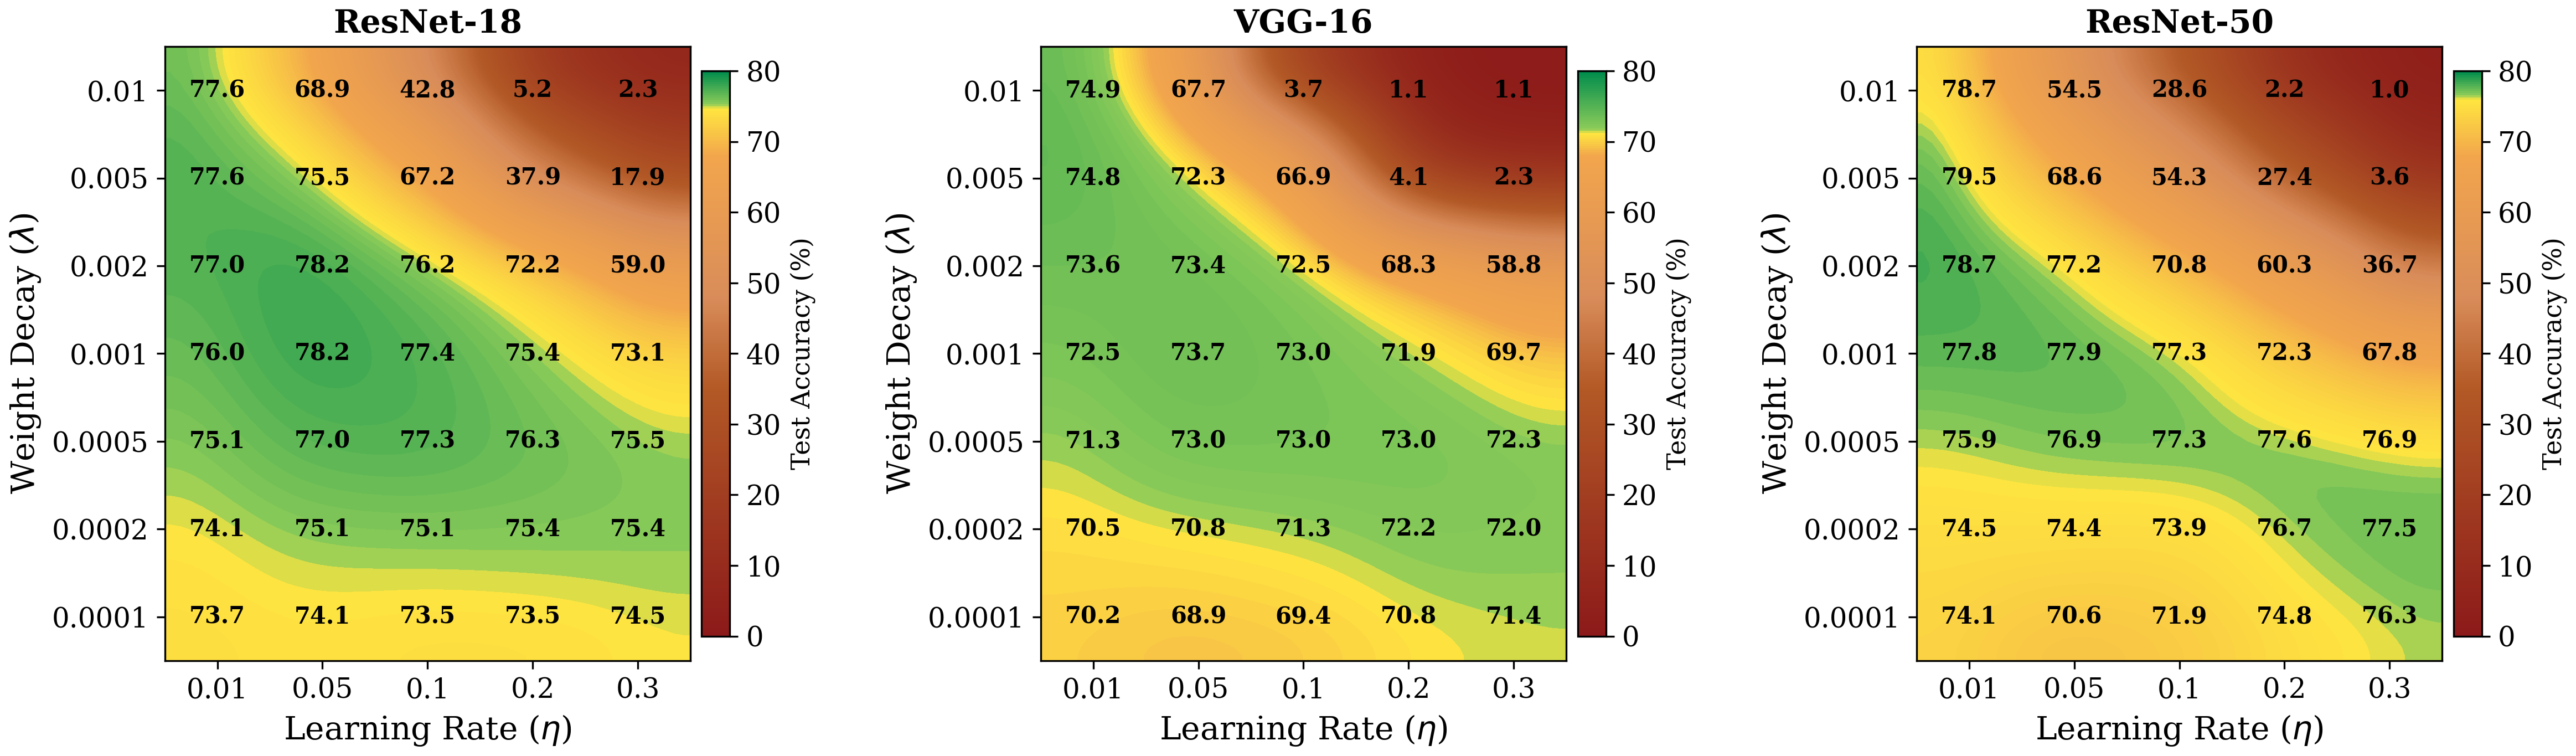
\includegraphics[width=\linewidth]{figures/appendix_exp2_3arch.png}
\caption{Exp.~2, full $\eta$--$\lambda$ heatmaps across architectures (SGDM, $B{=}128$). Cell value is the best test accuracy ($\%$) averaged over $2$--$4$ runs. The anti-diagonal high-accuracy band (i.e.\ $\eta\cdot\lambda\approx\text{const}$) is preserved on every architecture.}
\label{fig:robust-exp2}
\end{figure}

\paragraph{Exp.~3 -- Batch-size scaling with the linear LR rule.}
Under $\eta=0.1\times B/128$, the optimal $\lambda^{*}$ stays inside $[5\!\times\!10^{-4},\,10^{-3}]$ for all four batch sizes on all three architectures (Table~\ref{tab:robust-exp3}). At $B{=}64$ and $B{=}512$, all eight runs unanimously select $\lambda^{*}=10^{-3}$. Equivalently, the optimal joint product $\eta\cdot\lambda$ grows monotonically with $B$ on every architecture, in agreement with the batch-dependent scaling law $\lambda\approx B/(\eta n T_{epo})$ (Eq.~\eqref{coupling:Batch}).

\begin{table}[h]
\centering
\small
\caption{Cross-architecture comparison for Exp.~3, batch-size scaling under the linear LR rule $\eta=0.1\times B/128$. For each $B$ we report the optimal $\lambda^{*}$ and the corresponding peak test accuracy ($\%$, mean~$\pm$~half-range).}
\label{tab:robust-exp3}
\vspace{0.2em}
\begin{tabular}{c c c c c c c c}
\toprule
 & & \multicolumn{2}{c}{\textbf{ResNet-18}} & \multicolumn{2}{c}{\textbf{VGG-16}} & \multicolumn{2}{c}{\textbf{ResNet-50}} \\
\cmidrule(lr){3-4}\cmidrule(lr){5-6}\cmidrule(lr){7-8}
$B$ & $\eta$ & $\lambda^{*}$ & Acc.\ (\%) & $\lambda^{*}$ & Acc.\ (\%) & $\lambda^{*}$ & Acc.\ (\%) \\
\midrule
$64$  & $0.05$ & $1\!\times\!10^{-3}$ & $78.27 \pm 0.40$ & $1\!\times\!10^{-3}$ & $73.64 \pm 0.09$ & $5\!\times\!10^{-4}$ & $77.38 \pm 0.14$ \\
$128$ & $0.10$ & $1\!\times\!10^{-3}$ & $77.35 \pm 0.20$ & $1\!\times\!10^{-3}$ & $73.00 \pm 0.05$ & $1\!\times\!10^{-3}$ & $77.34 \pm 0.27$ \\
$256$ & $0.20$ & $5\!\times\!10^{-4}$ & $76.66 \pm 0.56$ & $1\!\times\!10^{-3}$ & $72.95 \pm 0.06$ & $5\!\times\!10^{-4}$ & $77.12 \pm 0.28$ \\
$512$ & $0.40$ & $1\!\times\!10^{-3}$ & $75.35 \pm 0.44$ & $1\!\times\!10^{-3}$ & $71.86 \pm 0.20$ & $5\!\times\!10^{-4}$ & $76.69 \pm 0.00$ \\
\bottomrule
\end{tabular}
\end{table}

\paragraph{Reproducibility summary.}
Across the $59$ $(\eta,\lambda)$ and $(B,\lambda)$ configurations of Exp.~2--3, the seed-to-seed difference $|\Delta(\text{seed}{=}123-\text{seed}{=}42)|$ is below $1\%$ for $76.3\%$ of configurations and below $2\%$ for $91.5\%$ of configurations; the residual five outliers all lie in unstable regimes (high $\eta\cdot\lambda$, near the divergence boundary). In the stable region the half-range is consistently below $0.5\%$. Combined with the architecture-level agreement reported above, this confirms that the three theoretical predictions of Section~\ref{sec:experiments}---(i) the stability boundary ordering, (ii) the inverse $\eta$--$\lambda$ relationship, and (iii) the batch-size coupling $\lambda\eta\propto B$---are robust to both random seed variation and the choice of architecture (residual vs.\ non-residual, shallow vs.\ deep).

